\documentclass[12pt]{article}
\usepackage{titlesec}
\usepackage{subcaption}
\usepackage[scaled]{helvet}  \renewcommand\familydefault{\sfdefault} % Font
\usepackage{graphicx} % Required for inserting images
\usepackage{geometry}
\usepackage{pgfplotstable}
\usepackage{amsmath}
\usepackage{enumitem}
\usepackage{tikz} 
\usetikzlibrary{petri,arrows.meta}
\geometry{a4paper, total={170mm,257mm},left=20mm, top=20mm,}
\usepackage[listings,breakable,skins]{tcolorbox}
% declare our code block environment
  \newtcblisting{tcbcodeblock}[1]{%
    enhanced,
    sharp corners,
    colframe=black,
    coltext=codefg,
    colback=codebg,
    breakable,
    size=fbox,
    listing only,
    listing options={%
      style=tcblatex,
      language={#1},
      showspaces=false,
      showstringspaces=false,
      commentstyle=\color{codegray},
      keywordstyle=\color{codegreen},
      stringstyle=\color{codecyan},
      basicstyle=\ttfamily\footnotesize
    }
  }
\renewcommand{\thesection}{\Roman{section}}
\renewcommand{\thesubsection}{\arabic{subsection}}
\renewcommand{\thesubsubsection}{\alph{subsubsection}.}

\titleformat{\section}{\normalfont\LARGE\bfseries}{\thesection.}{10pt}{}
\titleformat{\subsection}{\normalfont\Large}{\thesubsection.}{10pt}{}
\titleformat{\subsubsection}{\normalfont\large}{\thesubsubsection}{10pt}{}

\begin{document}
\thispagestyle{empty} %Suppress number of this page
\begin{center}
    \vspace{7pt}
    \fontsize{18pt}{17pt}\selectfont 
    \textbf{University of Science and Technology of Hanoi}
    \vspace{7pt}
\end{center}

\vspace{90pt}

\begin{center}
    \fontsize{30pt}{17pt}\selectfont 
    \textbf{Deep learning} 
    \vspace{50pt}

    \fontsize{20pt}{17pt}\selectfont 
    \textbf{Labwork 2}
    \vspace{50pt}


    \fontsize{17pt}{17pt}\selectfont
    \textbf{{Student id: }{2440057}}
    \vspace{15pt}

    \fontsize{17pt}{17pt}\selectfont
    \textbf{{Student name: }{Nguyen Nhat Anh}}
    \vspace{15pt}
    
\end{center}

\newpage
\section{Linear Regression using Gradient Descent}
\subsection{Mathematical Formulation}
The model assumes a linear relationship between $x$ (area) and $y$ (price):

\[
y = w_1 \cdot x + w_0
\]

The loss function used is Mean Squared Error (MSE):

\[
L = \frac{1}{2N} \sum_{i=1}^N (w_1 x_i + w_0 - y_i)^2
\]

The goal is to find the parameters $w_0$ and $w_1$ that minimize this loss using gradient descent.

\subsection{Gradient Descent}

The partial derivatives of the loss with respect to each parameter are:

\[
\frac{\partial L}{\partial w_0} = \frac{1}{N} \sum_{i=1}^N (w_1 x_i + w_0 - y_i)
\]

\[
\frac{\partial L}{\partial w_1} = \frac{1}{N} \sum_{i=1}^N x_i (w_1 x_i + w_0 - y_i)
\]

And the update rules are:

\[
w_0 = w_0 - r \cdot \frac{\partial L}{\partial w_0}, \quad w_1 = w_1 - r \cdot \frac{\partial L}{\partial w_1}
\]

Where $r$ is the learning rate.

\subsection{Python Implementation}

\begin{verbatim}
def load_data(filename):
    x_vals = []
    y_vals = []
    with open(filename, 'r') as file:
        for line in file:
            parts = line.strip().split(',')
            x_vals.append(float(parts[0]))
            y_vals.append(float(parts[1]))
    return x_vals, y_vals
    
def compute_loss(x_vals, y_vals, w0, w1):
    N = len(x_vals)
    total = 0.0
    for i in range(N):
        y_pred = w1 * x_vals[i] + w0
        total += (y_pred - y_vals[i]) ** 2
    return 0.5 * total / N

def linear_regression(x_vals, y_vals, lr=0.0001, threshold=1e-3, max_iter=10000):
    w0, w1 = 0.0, 1.0
    N = len(x_vals)

    for it in range(max_iter):
        dw0 = 0.0
        dw1 = 0.0
        for i in range(N):
            error = (w1 * x_vals[i] + w0) - y_vals[i]
            dw0 += error
            dw1 += error * x_vals[i]
        dw0 /= N
        dw1 /= N

        w0 -= lr * dw0
        w1 -= lr * dw1

        loss = compute_loss(x_vals, y_vals, w0, w1)

        if it % 100 == 0:
            print(f"Iter {it}: w0 = {w0:.4f}, w1 = {w1:.4f}, loss = {loss:.4f}")

        if loss < threshold:
            break
    return w0, w1
\end{verbatim}

\subsection{Final Result}
After training the model using the dataset:

\begin{verbatim}
10,55
20,80
40,100
60,120
80,150
\end{verbatim}

\noindent 
The final weights obtained were:

\begin{verbatim}
w0 = 11.405874100931408, w1 = 1.8971592390207914
\end{verbatim}

\subsection{Visualization}
The figure below shows the original data points and the fitted regression line.

\begin{center}
    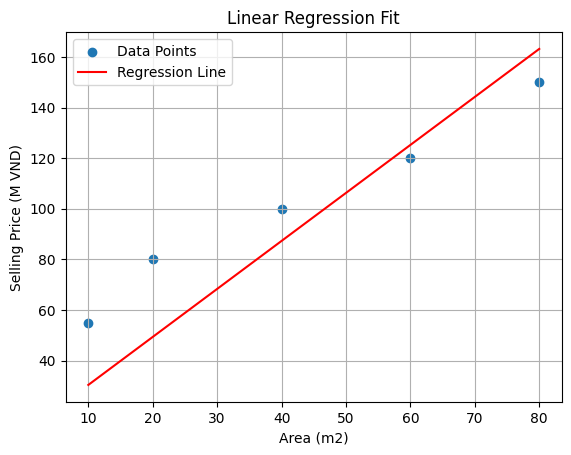
\includegraphics[scale=0.7]{output.png}
\end{center}

\subsection{Analysis of Learning Rate}
The learning rate affects convergence speed and stability.

\begin{itemize}
    \item With a small learning rate (e.g., 0.0001), the model converges slowly but stably.
    \item A large learning rate (e.g., 0.1) may lead to faster convergence but risks overshooting.
    \item A suitable learning rate balances speed and accuracy.
\end{itemize}

\subsection{Conclusion}
This lab demonstrates how gradient descent can be used to solve a simple linear regression problem from scratch. The final result fits the data well and shows how adjusting the learning rate influences the convergence behavior.

\end{document}